\documentclass[hyperref]{article}
%MS%%%%%%%%%%%%%%%%%%%% Article Format %%%%%%%%%%%%%%%%%
%+++++++++++++++++++++ Usepackage +++++++++++++++%%
\usepackage{graphicx} %% Package for Figure
\usepackage{float} %% Package for Float
\usepackage{amssymb}
\usepackage{amsmath}
\usepackage{mathtools}
\usepackage[thmmarks,amsmath]{ntheorem} %% If amsmath is applied, then amsma is necessary
\usepackage{bm} %% Bold Mathematical Symbols
\usepackage[colorlinks,linkcolor=cyan,citecolor=cyan]{hyperref}
\usepackage{extarrows}
\usepackage[hang,flushmargin]{footmisc} %% Let the footnote not indentation
\usepackage[square,comma,sort&compress,numbers]{natbib} %% Sort of References
\usepackage{mathrsfs} %% Swash letter
\usepackage[font=footnotesize,skip=0pt,textfont=rm,labelfont=rm]{caption,subcaption} 
%% Format of Caption for Tab. and Fig.
\usepackage{booktabs} %% tables with three lines
\usepackage{tocloft}
\usepackage{graphicx}

\usepackage{algorithm}  
%\usepackage{algorithmicx}  
\usepackage{algorithmic}
%+++++++++++++++ Proof etc. +++++++++++++++++++++++++%%
{%% Environment of Proof
	\theoremstyle{nonumberplain}
	\theoremheaderfont{\bfseries}
	\theorembodyfont{\normalfont}
	\theoremsymbol{\mbox{$\Box$}}
	\newtheorem{proof}{Proof}
}

\usepackage{theorem}
\newtheorem{theorem}{Theorem}[section]
\newtheorem{lemma}{Lemma}[section]
\newtheorem{definition}{Definition}[section]
\newtheorem{assumption}{Assumption}[section]
\newtheorem{example}{Example}[section]
\newtheorem{corollary}{Corollary}[section]
{%% Environment of Remark
	\theoremheaderfont{\bfseries}
	\theorembodyfont{\normalfont}
	\newtheorem{remark}{Remark}[section]
}
\usepackage{abstract}
\renewcommand{\abstractnamefont}{\Large\bfseries}
%\numberwithin{equation}{section} %% Number of Equation
%++++++++++++++++++++++++++++++++ Page format ++++++++++++++++++++++++++%%
\graphicspath{{figure/}}                                 %% Path of Figures
\usepackage[a4paper]{geometry}                           %% Paper size
\geometry{left=2.5cm,right=2.5cm,top=2.5cm,bottom=2.5cm} %% Margin
\linespread{1.2}      
\usepackage{cite}

% matlab code package
\usepackage{appendix}
\usepackage{listings}%插入代码
\usepackage{color}
\lstset{%代码格式的配置
	extendedchars=false,            % Shutdown no-ASCII compatible
	language=Matlab,                % !!!选择代码的语言
	basicstyle=\footnotesize\tt,    % the size of the fonts that are used for the code
	tabsize=3,                            % sets default tabsize to 3 spaces
	numbers=left,                   % where to put the line-numbers
	numberstyle=\tiny,              % the size of the fonts that are used for the line-numbers
	stepnumber=1,                   % the step between two line-numbers. If it's 1 each line
	% will be numbered
	numbersep=5pt,                  % how far the line-numbers are from the code   %
	keywordstyle=\color[rgb]{0,0,1},                % keywords
	commentstyle=\color[rgb]{0.133,0.545,0.133},    % comments
	stringstyle=\color[rgb]{0.627,0.126,0.941},      % strings
	backgroundcolor=\color{white}, % choose the background color. You must add \usepackage{color}
	showspaces=false,               % show spaces adding particular underscores
	showstringspaces=false,         % underline spaces within strings
	showtabs=false,                 % show tabs within strings adding particular underscores
	frame=single,                   % adds a frame around the code
	captionpos=b,                   % sets the caption-position to bottom
	breaklines=true,                % sets automatic line breaking
	breakatwhitespace=false,        % sets if automatic breaks should only happen at whitespace
	title=\lstname,                 % show the filename of files included with \lstinputlisting;
	% also try caption instead of title
	mathescape=true,escapechar=?    % escape to latex with ?..?
	escapeinside={\%*}{*)},         % if you want to add a comment within your code
	%columns=fixed,                  % nice spacing
	%morestring=[m]',                % strings
	%morekeywords={%,...},%          % if you want to add more keywords to the set
	%    break,case,catch,continue,elseif,else,end,for,function,global,%
	%    if,otherwise,persistent,return,switch,try,while,...},%
}
\usepackage{enumitem}
% \setlength{\parskip}{0.4em}


                                   %% Line Spread
%MS%%%%%%%%%%%%%%%%%%%%%%%%%%%% End Format %%%%%%%%%%%%%%%%%%%%%%%%%%%%%%%%%%

%MS%%%%%%%%%%%%%%%%%%%%%%%%%%%%%%%%%%%%%%%%%%%
%MS                                         %%
%MS        The Main Body begins here        %%
%MS                                         %%
%MS%%%%%%%%%%%%%%%%%%%%%%%%%%%%%%%%%%%%%%%%%%%

%MS++++++++++++++++++++++++++++++ Title +++++++++++++++++++
\title{ME5413 Autonomous Mobile Robotics: \\ Homework 2}
\author{\textup{Chen Yihui \ \ \ A0263115N \\ Wang Renjie \ A0263387U }}
\begin{document}
	\begin{titlepage}
		\center
		\newcommand{\HRule}{\rule{\linewidth}{0.5mm}}
		
\includegraphics[width=8cm]{logo.png}\\[1cm] 
		\quad\\[2cm]
		\textsl{\Large National University of Singapore}\\[0.5cm] 
		\textsl{\large College of Design and Engineering}\\[0.5cm]
		\makeatletter
		\HRule \\[0.4cm]
		{ \huge \bfseries \@title}\\[0.4cm] 
		\HRule \\[2cm]
		\begin{minipage}{0.4\textwidth}
			\begin{flushleft} \large
				\emph{Group 9:}\\
				\@author 
			\end{flushleft}
		\end{minipage}
		~
		\begin{minipage}{0.4\textwidth}
			\begin{flushright} \large
				\emph{Supervisor:} \\
				\textup{Prof. Marcelo H Ang Jr}
			\end{flushright}
		\end{minipage}\\[3cm]
		\makeatother
		%{\large \emph{Matriculation Number: A0263115N}}\\[0.5cm]
		{\large \emph{Email Address: e1010473@u.nus.edu \\	\ \ \ \ \ \ \ \ \ \ \ \ \ \ \ \ \ \ \ \ e1010745@u.nus.edu}}\\[0.5cm]
		{\large \today}\\[2cm] 
		\vfill 
	\end{titlepage}

\section{Task 1: ICP Algorithm for Matched Point Cloud}

\hspace{1.0em}

In Task 1, we assume the correspondence is known for the two point clouds and perform ICP algorithm to do point cloud registration. Firstly, the SVD-based ICP algorithm is reviewed. 

Given the source point cloud $X=\{x_{1}, x_{2}, ..., x_{m}\}$ and target point cloud $Y=\{y_{1}, y_{2}, ..., y_{m}\}$, the task for point cloud registration is to find a rotation matrix $R$ and a translation matrix $t$ that can transform $X$ to $Y$. In other words, we need to find $R$ and $t$ to minimize the sum of the squared distance between the corresponding points in the two point clouds:

\begin{equation}
\begin{aligned}
E(R,t)&=\frac{1}{m}\sum_{i=1}^{m}\left \| y_{i}-Rx_{i}-t \right \|^{2}\\
&=\frac{1}{m}\sum_{i=1}^{m}(\left \| y_{i}-u_{y}-R(x_{i}-u_{x})\right \|^{2}+\left \| u_{y}-Ru_{x}-t\right \|^{2})
\label{eq1}
\end{aligned}
\end{equation}

where $u_{x}$ and $u_{y}$ are the centroid of the point set $X$ and $Y$, $u_{x}=\frac{1}{m}\sum_{i=1}^{m}x_{i}$ and $u_{y}=\frac{1}{m}\sum_{i=1}^{m}y_{i}$. To simplify the problem, we divide Eq.~\ref{eq1} to:

\begin{equation}
\begin{aligned}
E_{1}(R,t)=\frac{1}{m}\sum_{i=1}^{m}\left \| y_{i}-u_{y}-R(x_{i}-u_{x})\right \|^{2}, \ \ \
E_{2}(R,t)=\left \| u_{y}-Ru_{x}-t  \right \|^{2}
\label{eq2}
\end{aligned}
\end{equation}

Therefore, we can first find the $R$ to minimize $E_{1}(R,t)$ and then calculate $t$ from $E_{2}(R,t)$. Suppose $x_{i}^{'}=x_{i}-u_{x}$, $y_{i}^{'}=y_{i}-u_{y}$, the problem turns to:

\begin{equation}
\begin{aligned}
min\{E_{1}(R,t)\}=min\{\frac{1}{m}\sum_{i=1}^{m}(y_{i}^{'T}y_{i}^{'}+x_{i}^{'T}R^{T}Rx_{i}^{'}-2y_{i}^{'T}Rx_{i}^{'})\} = max \{\sum_{i=1}^{m}y_{i}^{'T}Rx_{i}^{'}\}
\label{eq3}
\end{aligned}
\end{equation}

Using the properties of trace, we derive:

\begin{equation}
\begin{aligned}
\sum_{i=1}^{m}y_{i}^{'T}Rx_{i}^{'}=\sum_{i=1}^{m}Trace(y_{i}^{'T}Rx_{i}^{'})=Trace(\sum_{i=1}^{m}Rx_{i}^{'}y_{i}^{'T})=Trace(RH)
\label{eq4}
\end{aligned}
\end{equation}

where $H=\sum_{i=1}^{m}x_{i}^{'}y_{i}^{'T}$. According to Schwarz inequality, we can maximum Eq.~\ref{eq4} by finding a $R$ that can convert $RH$ to the form of $AA^{T}$. Therefore, we apply Singular Value Decomposition (SVD) on $H$ and get $H=U\Sigma V^{T}$. Then we choose the rotation matrix:

\begin{equation}
\begin{aligned}
R=VU^{T} 
\label{eq5}
\end{aligned}
\end{equation}

Then, $RH=VU^{T}U\Sigma V^{T}=V\Sigma V^{T}=V\Sigma^{1/2}(V\Sigma^{1/2})^{T}$, which is in the form of $AA^{T}$ and we finally minimize $E_{1}(R,t)$. After obtaining $R$, we can solve the translation matrix $t$ to minimize $E_{2}(R,t)$:

\begin{equation}
\begin{aligned}
t=u_{y}-Ru_{x} 
\label{eq6}
\end{aligned}
\end{equation}

Since we have known the corresponding point pairs between source point cloud $X$ and target $Y$, we can easily get the homogeneous transformation matrix $T\in SE(3)$ by combing the rotation matrix $R\in SO(3)$ and translation matrix $t \in \mathbb{R}^{3}$ computed in Eq.~\ref{eq5} and \ref{eq6}:

\begin{equation}
\begin{aligned}
T=\begin{pmatrix}
R &t \\ 
0^{T} &1 
\end{pmatrix}
\label{eq7}
\end{aligned}
\end{equation}

The core code of ICP algorithm with comment is shown in Fig.~\ref{fig1a} and derived transformation matrix $T$ is recorded in Fig.~\ref{fig1b}. As is shown in Fig.~\ref{fig1c}, the source point cloud (red) is transformed to the blue one, which is overlapped with the target point cloud (green). The final mean error between the blue and green point clouds is about 0.226. 


\begin{figure}[H]
	\centering
	\begin{minipage}[t]{0.32\textwidth}
		\centering
		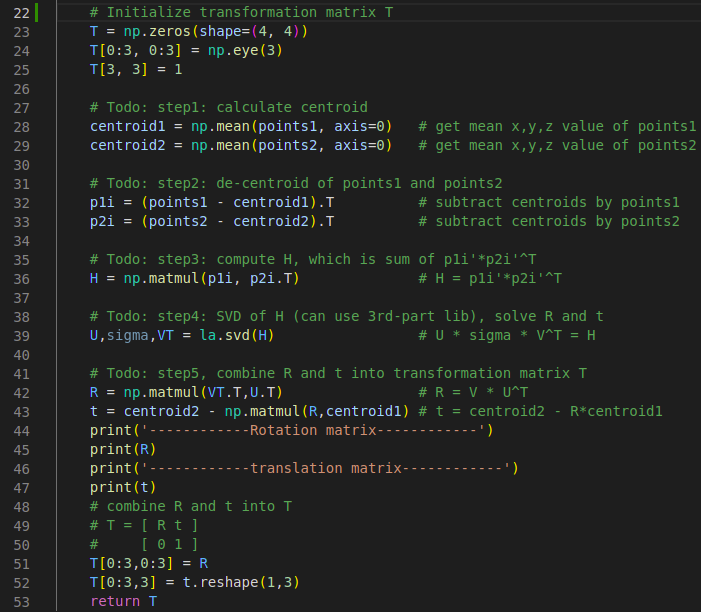
\includegraphics[width=4cm]{1_code.png}
		\subcaption{Core code for ICP algorithm}
		\label{fig1a}
	\end{minipage}
	\begin{minipage}[t]{0.32\textwidth}
		\centering
		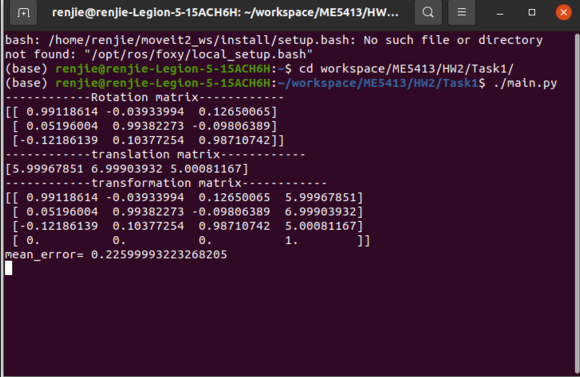
\includegraphics[width=5cm]{1_T.png}
		\subcaption{Derived transformation matrix $T$}
		\label{fig1b}
	\end{minipage}
	\begin{minipage}[t]{0.32\textwidth}
		\centering
		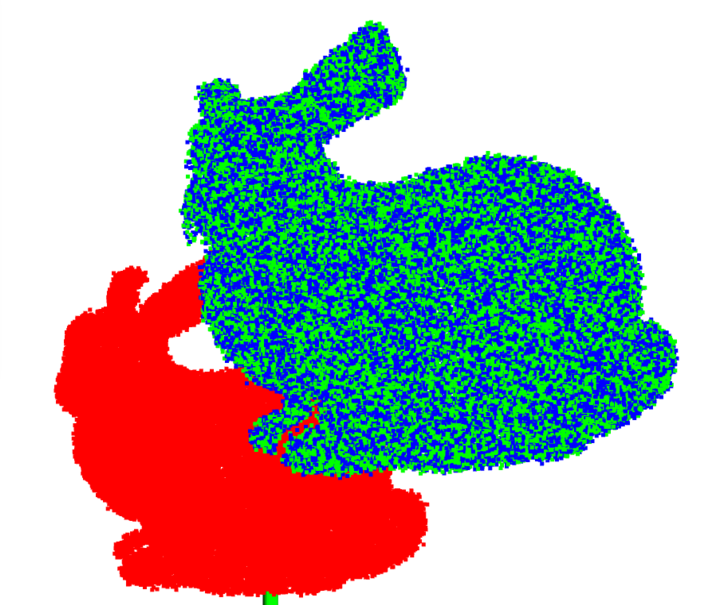
\includegraphics[width=5cm]{1_result.png}
		\subcaption{Visualization result}
		\label{fig1c}
	\end{minipage}
	\caption{Implementation of ICP algorithm for matched point cloud}
	\label{fig1}
\end{figure} 


\section{Task 2: ICP Algorithm for Unmatched Point Cloud}

\hspace{1.0em}

In real cases, the correspondence between the source and target point cloud is usually unknown. A common method is to regard the nearest neighbor point as corresponding point and solve the problem iteratively. The ICP algorithm for unmatched point cloud is given in Alg.~\ref{alg:algorithm1}.

\begin{algorithm}
	\caption{SVD-based ICP algorithm for unmatched point cloud}
	\begin{algorithmic}  
		\STATE Initialize the accumulated transformation matrix $T\_accumulated$.
		\WHILE {$error > threshold$}
		
		\STATE Step 1: Find the corresponding points from two point clouds.
		
		\STATE Step 2: Compute the transformation matrix $T$ following the steps in Task 1.
		
		\STATE Step 3: Update accmulated matrix. \ ($T\_accumulated=T*T\_accumulated$)
		
		\STATE Step 4: Apply alignment. \ ($x_{i}^{'}=T*x_{i}$)
		
		\STATE Step 5: Update error.
		
		\ENDWHILE
		
	\end{algorithmic}
	\label{alg:algorithm1} 
\end{algorithm}

The $threshold$ is set to be 0.1 and core code for the iterative ICP algorithm is shown in Fig.~\ref{fig2}. To show the more and more overlapped rabits, we record the transformation matrix $T$ and $T\_accumulated$ in iteration 7, 15 and 23, as well as visualizing the two point clouds and mean error between them (Fig.~\ref{fig3}). 

\begin{figure}[H]
	\centering
		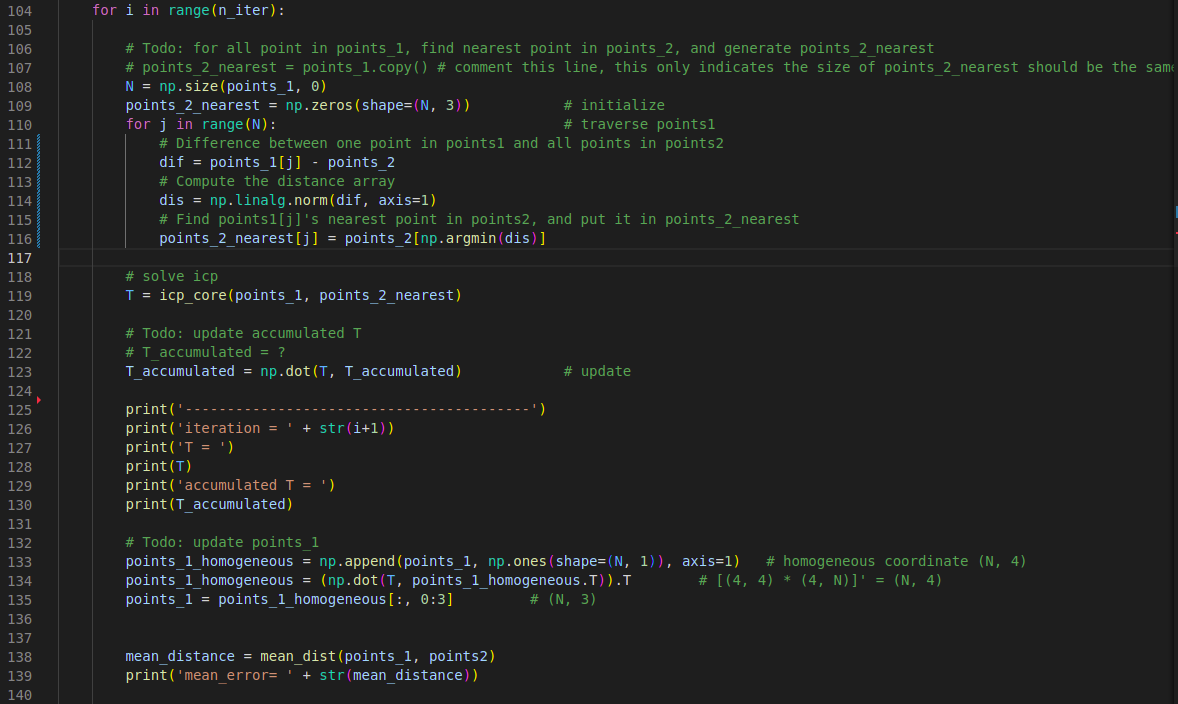
\includegraphics[width=6cm]{2_code.png}
	\caption{Code for ICP algorithm with unmatched point cloud}
	\label{fig2}
\end{figure} 

\begin{figure}[H]
	\centering
	\begin{minipage}[t]{0.32\textwidth}
		\centering
		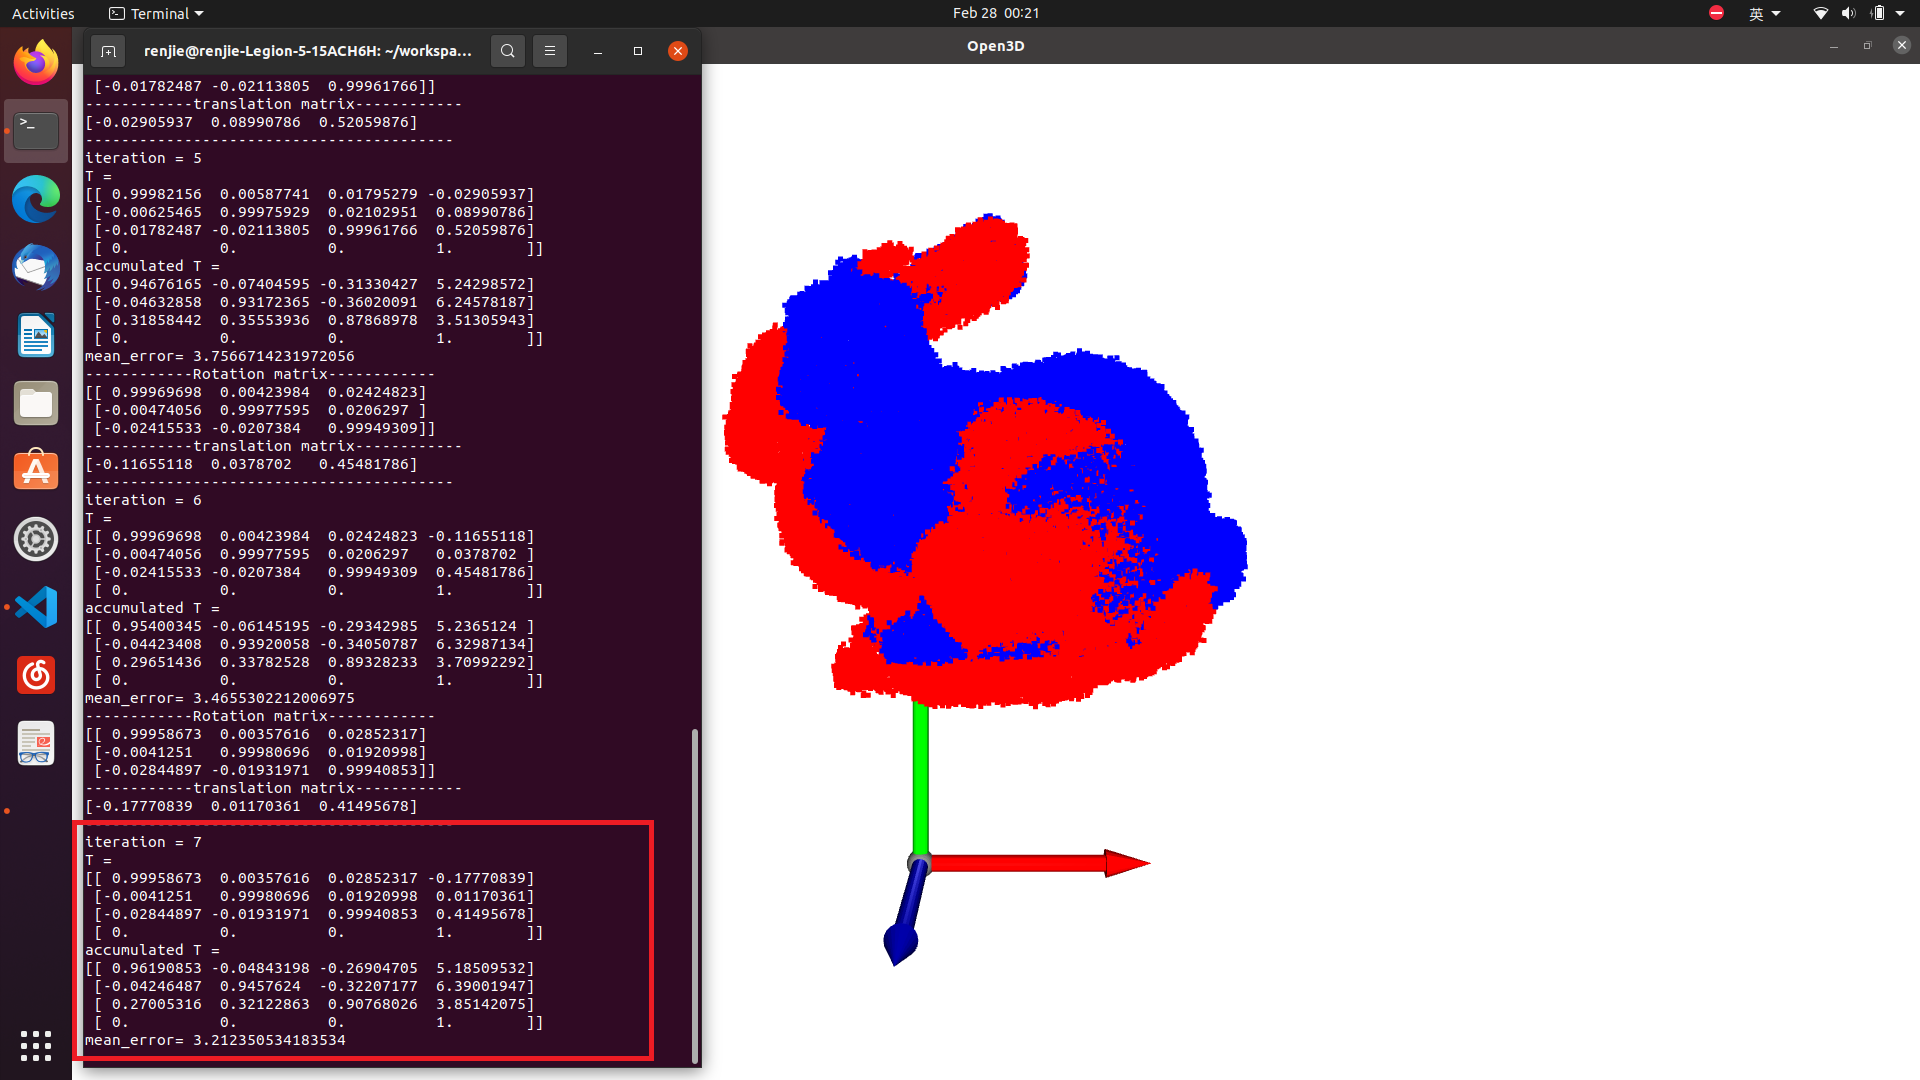
\includegraphics[width=5cm]{2_M1.png}
		\subcaption{Results at iteration 7}
		\label{fig3a}
	\end{minipage}
	\begin{minipage}[t]{0.32\textwidth}
		\centering
		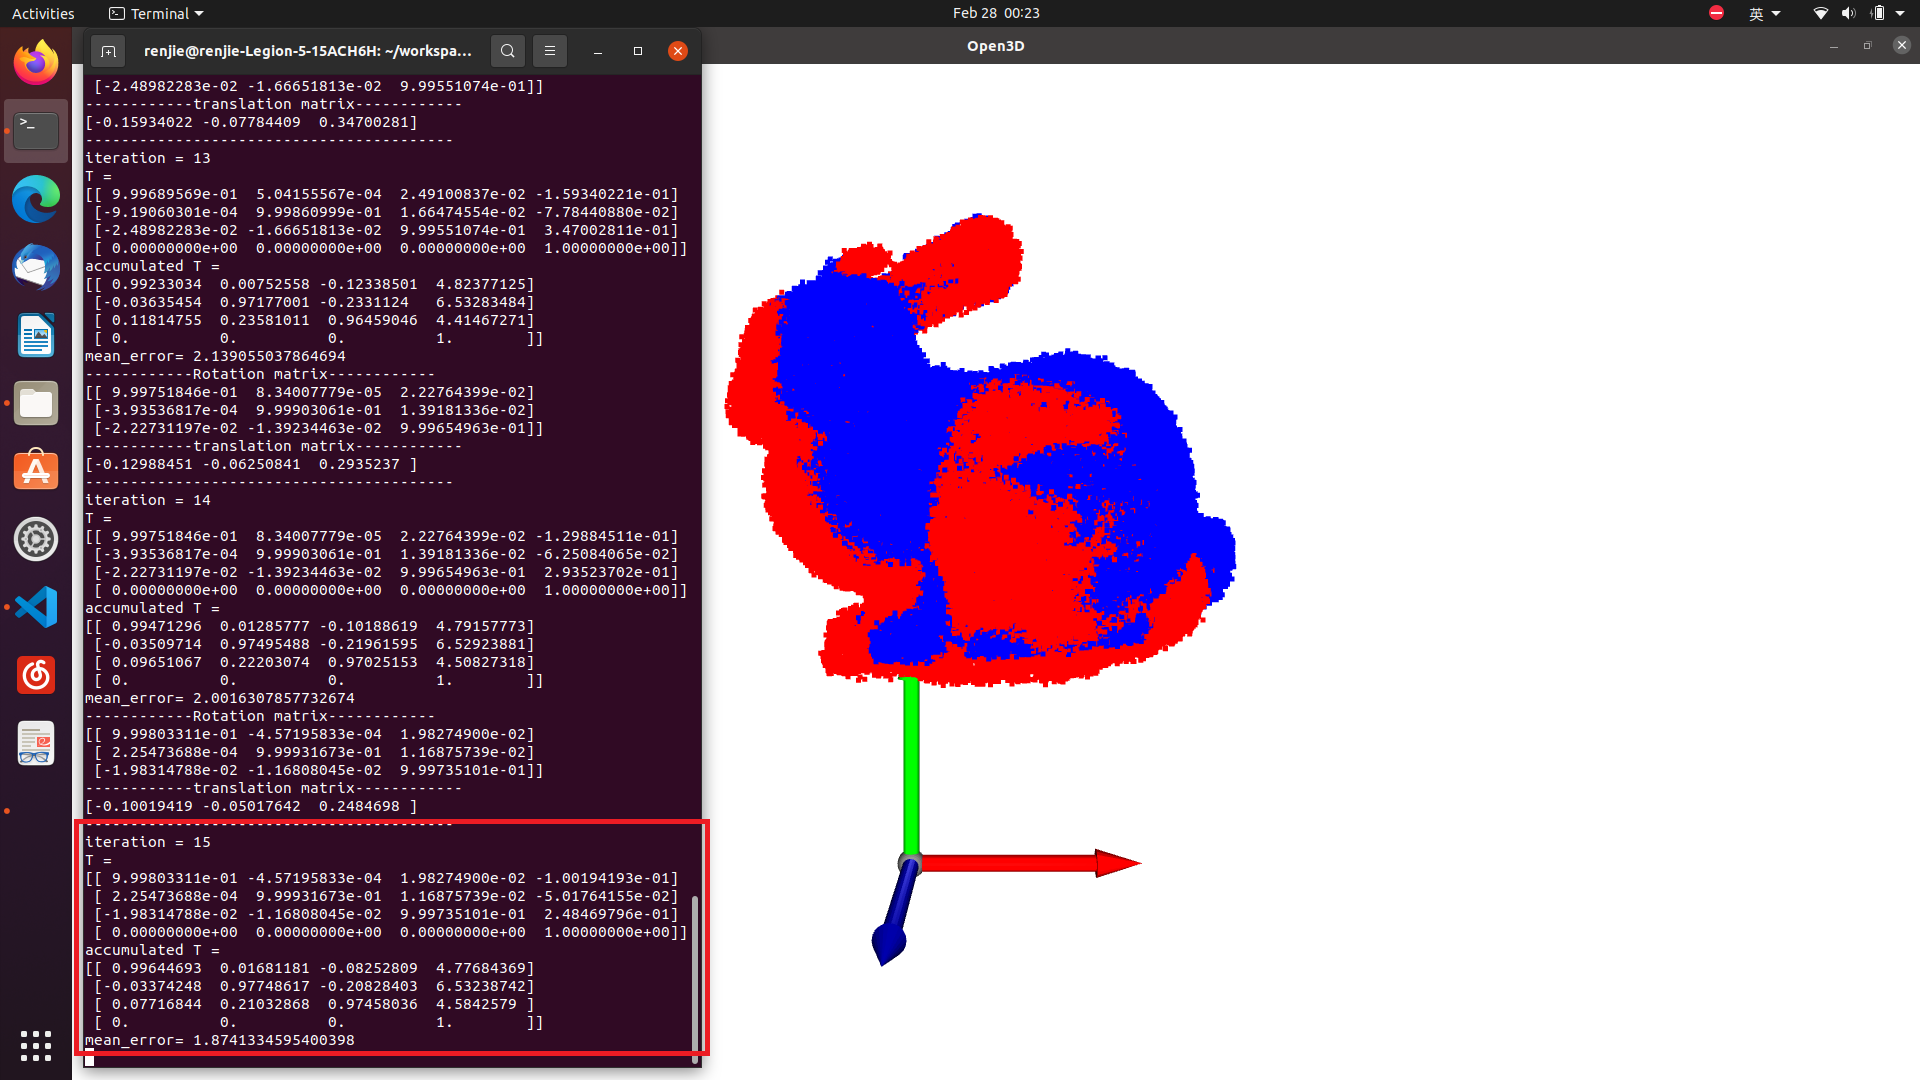
\includegraphics[width=5cm]{2_M2.png}
		\subcaption{Results at iteration 15}
		\label{fig3b}
	\end{minipage}
	\begin{minipage}[t]{0.32\textwidth}
		\centering
		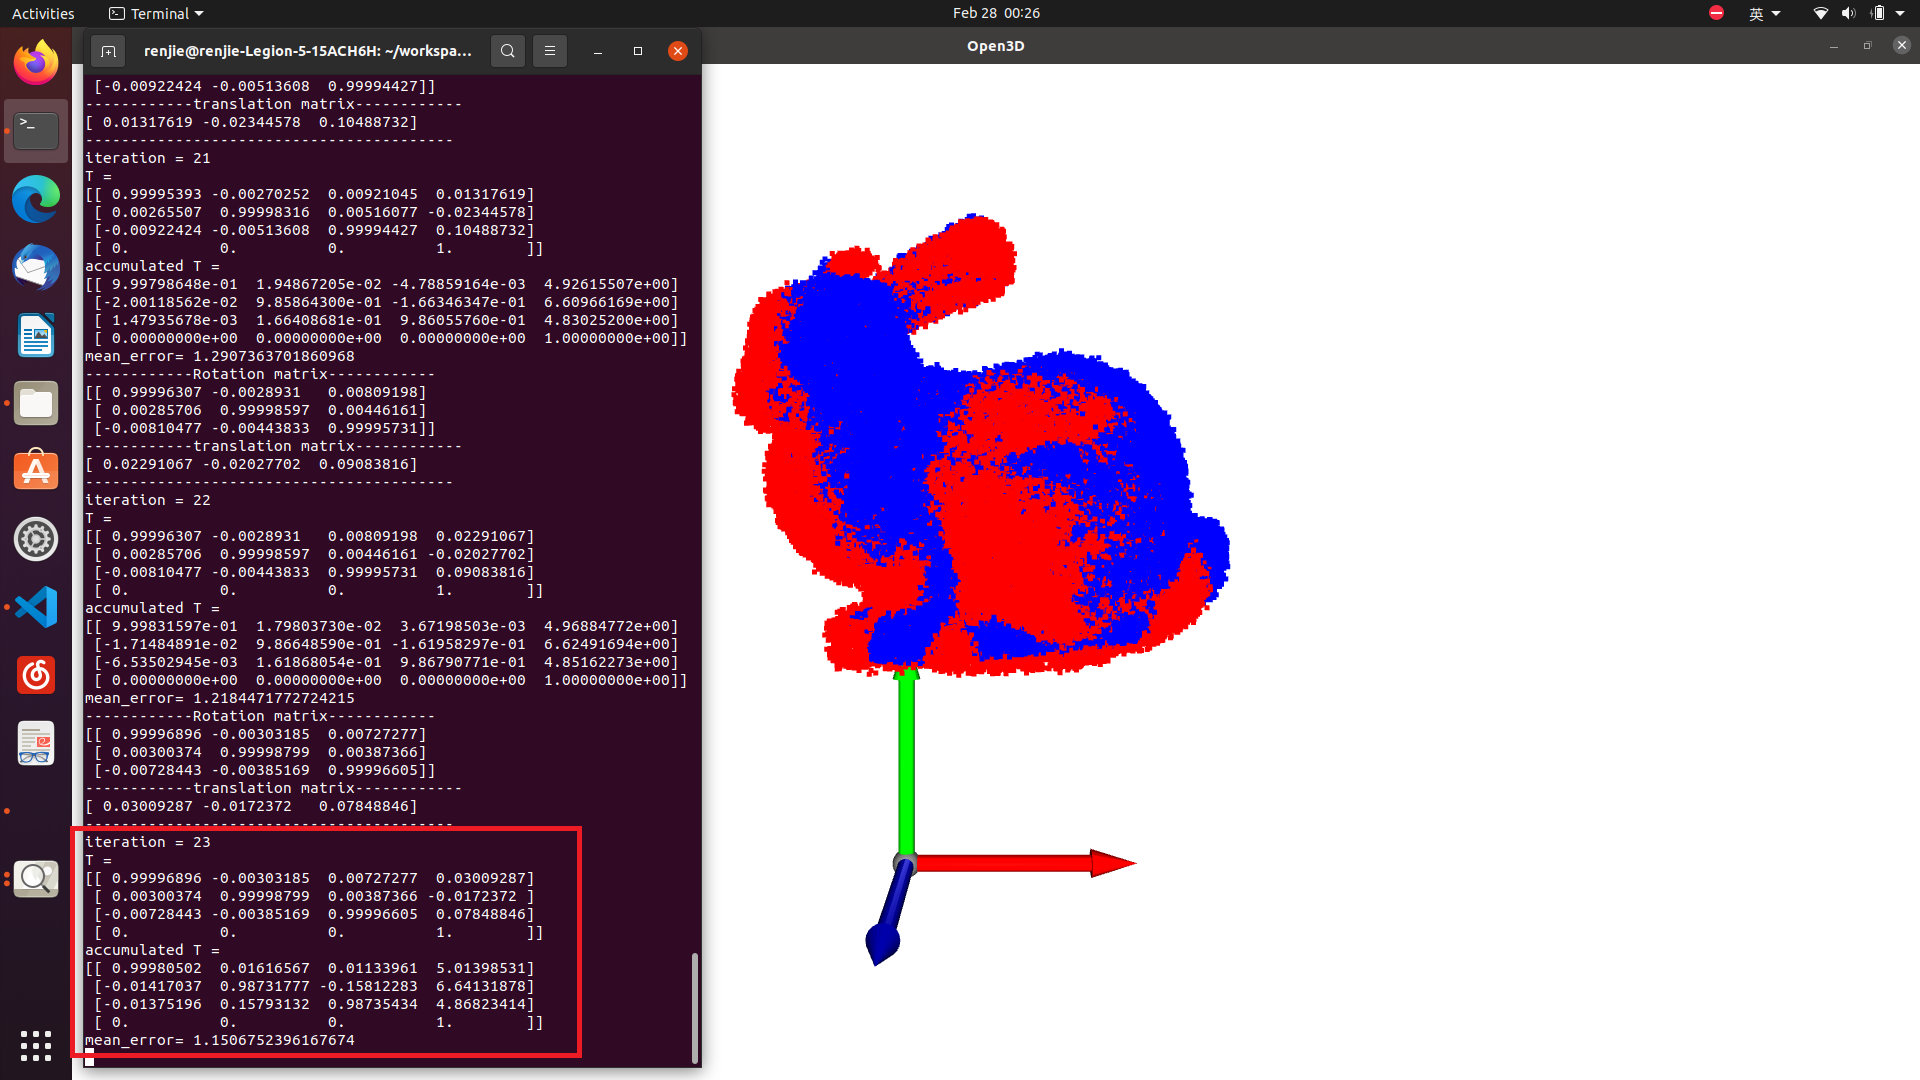
\includegraphics[width=5cm]{2_M3.png}
		\subcaption{Results at iteration 23}
		\label{fig3c}
	\end{minipage}
	\caption{Implementation of ICP algorithm for unmatched point cloud}
	\label{fig3}
\end{figure} 

We can see the mean error is reduced after each iteration (3.212 to 1.874 to 1.151), and it declines more and more slowly as iteration number increases. The final result at 30th iteration is shown in Fig.~\ref{fig4}, where the mean error is about 0.797 and still higher than the mannually set threshold. We increase the maximum iteration number to 50 and the result is shown in Fig.~\ref{fig4b}. The mean error is only ? now and the accumulated transformation matrix $T\_accumulated$ is very close to that we derived in Task1. However, the cost time is rather high (650s) because of the time-consuming corresponding points search procedure. In practice, kd-tree can be used to search for the nearest points more efficiently. Moreover, some learning-based methods have been popular for solving the point cloud registration problem. 

\begin{figure}[H]
	\centering
	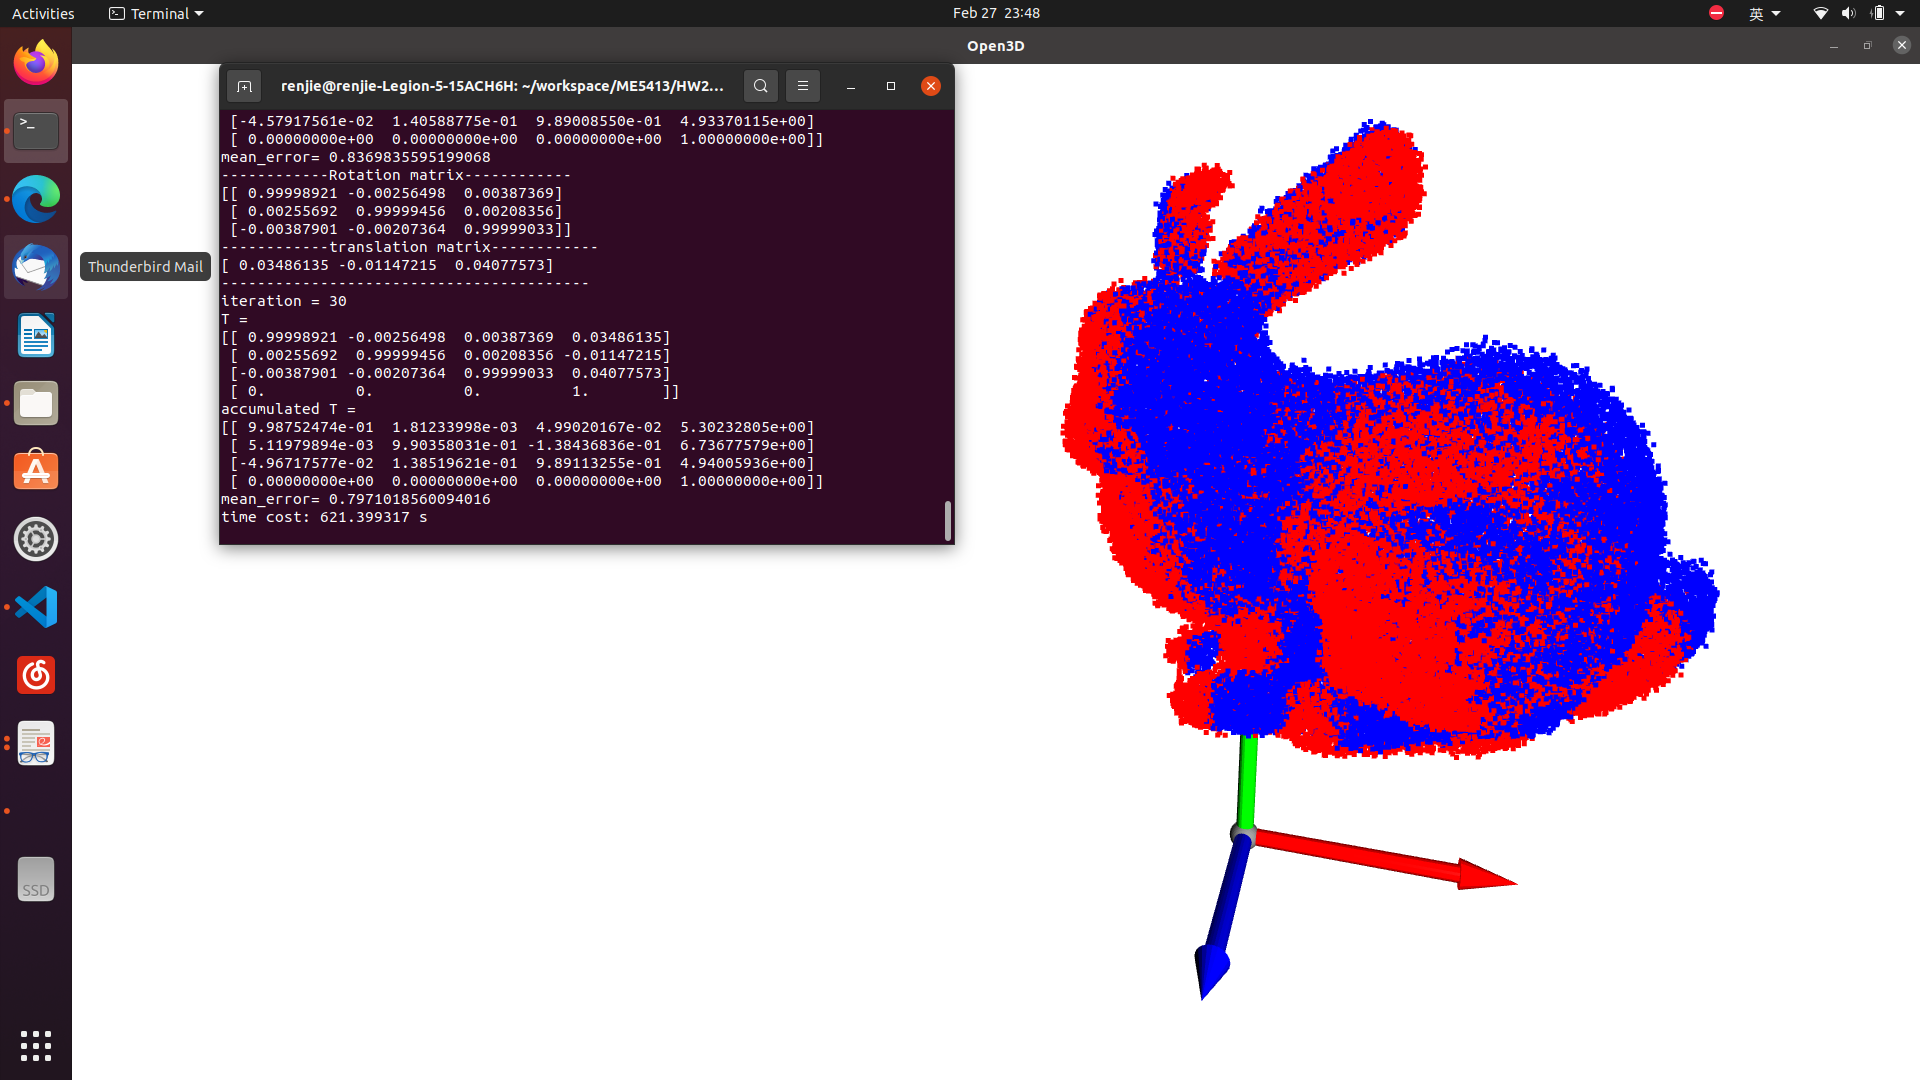
\includegraphics[width=6cm]{2.3.png}
	\caption{Code for ICP algorithm with unmatched point cloud}
	\label{fig4}
\end{figure}






\section{Task 3: Running SLAM Algorithms}

\subsection{Cartographer for 2D LiDAR SLAM}

\hspace{1.0em}
Cartographer is an open-source, real-time, simultaneous localization and mapping (SLAM) system developed by Google. It is designed to create high-resolution maps of indoor and outdoor environments using data collected from a variety of sensors, including LiDAR, IMU, and cameras. Here we apply the algorithm to do 2D mapping using the collected data in the given rosbag ('\textless 2dlidar.bag \textgreater'). 

After compiling the Cartographer on ROS Noetic, we need to configure the .lua and .lauch file to run the algorithm on our own rosbag. First we check the topics in the given rosbag and use "rqt\_graph" and "rqt\_tf\_tree" to plot the node diagram and tf structure. Then we need to change some important parameters:

\begin{itemize}[itemsep=3pt,topsep=0pt,parsep=0pt]
	\item We set $published\_frame$ to "odom" and set the flag $use\_odometry$ "true".
	\item Since we only have one lidar, we set $num\_laser\_scans=1, \ num\_multi\_echo\_laser\_scans = 0$.
	\item We also need to set $TRAJECTORY\_BUILDER\_2D.use\_imu\_data = false$ since we haven't applied imu.
\end{itemize}

As for the .launch file, we start recording a new rosbag before the algorithm starts for evaluating the performance afterwards. We include our .lua configuration and start rviz for visualization. The whole .lua and launch file is included in the appendix. The mapping process visualized by rviz is shown in Fig.~\ref{fig5}, where we can see the loop closure can adjust the map to achieve better results.


\begin{figure}[H]
	\centering
	\begin{minipage}[t]{0.32\textwidth}
		\centering
		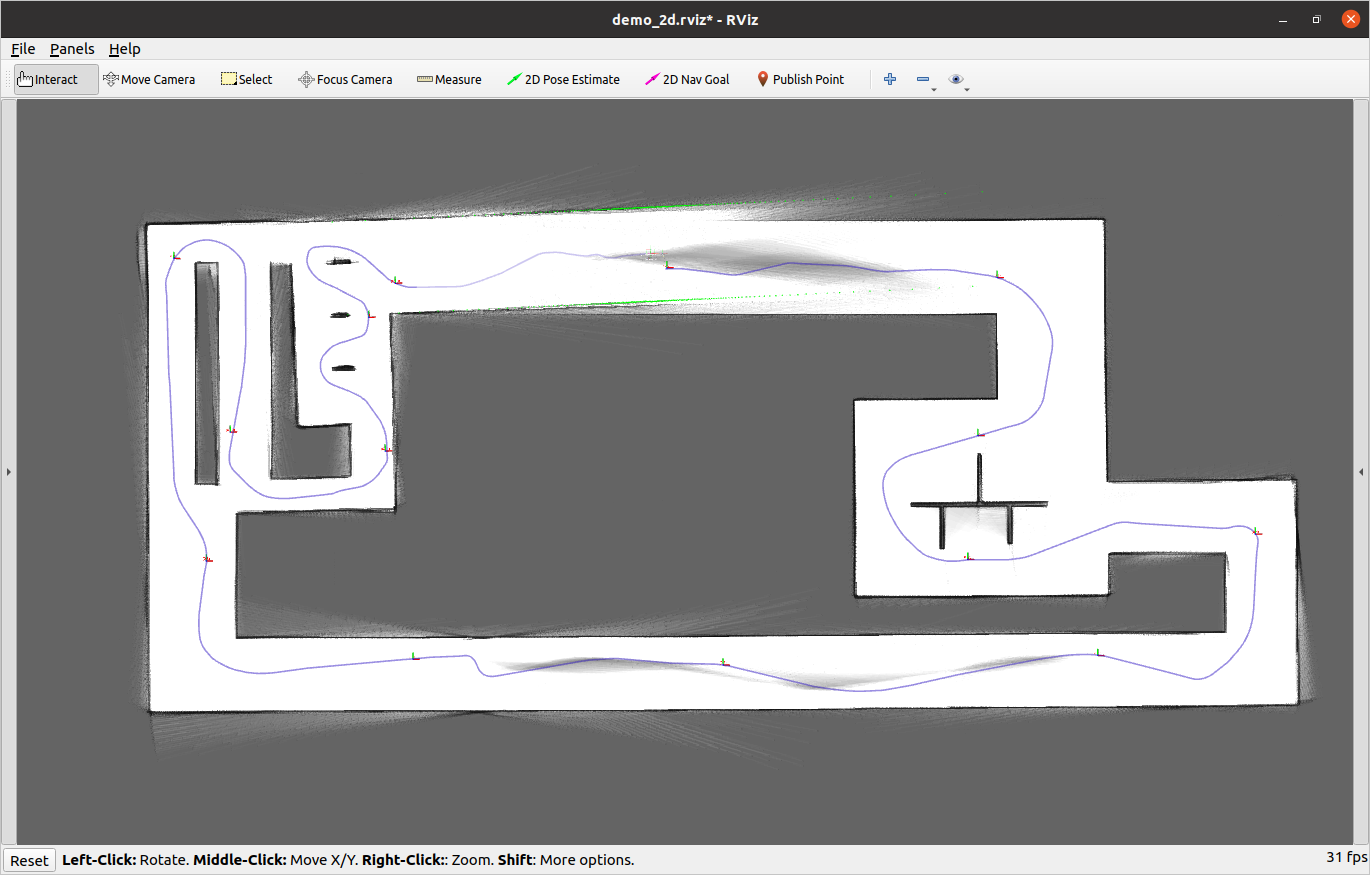
\includegraphics[width=5cm]{task3a_result1.png}
		\subcaption{Before reaching the start point}
		\label{fig5a}
	\end{minipage}
	\begin{minipage}[t]{0.32\textwidth}
		\centering
		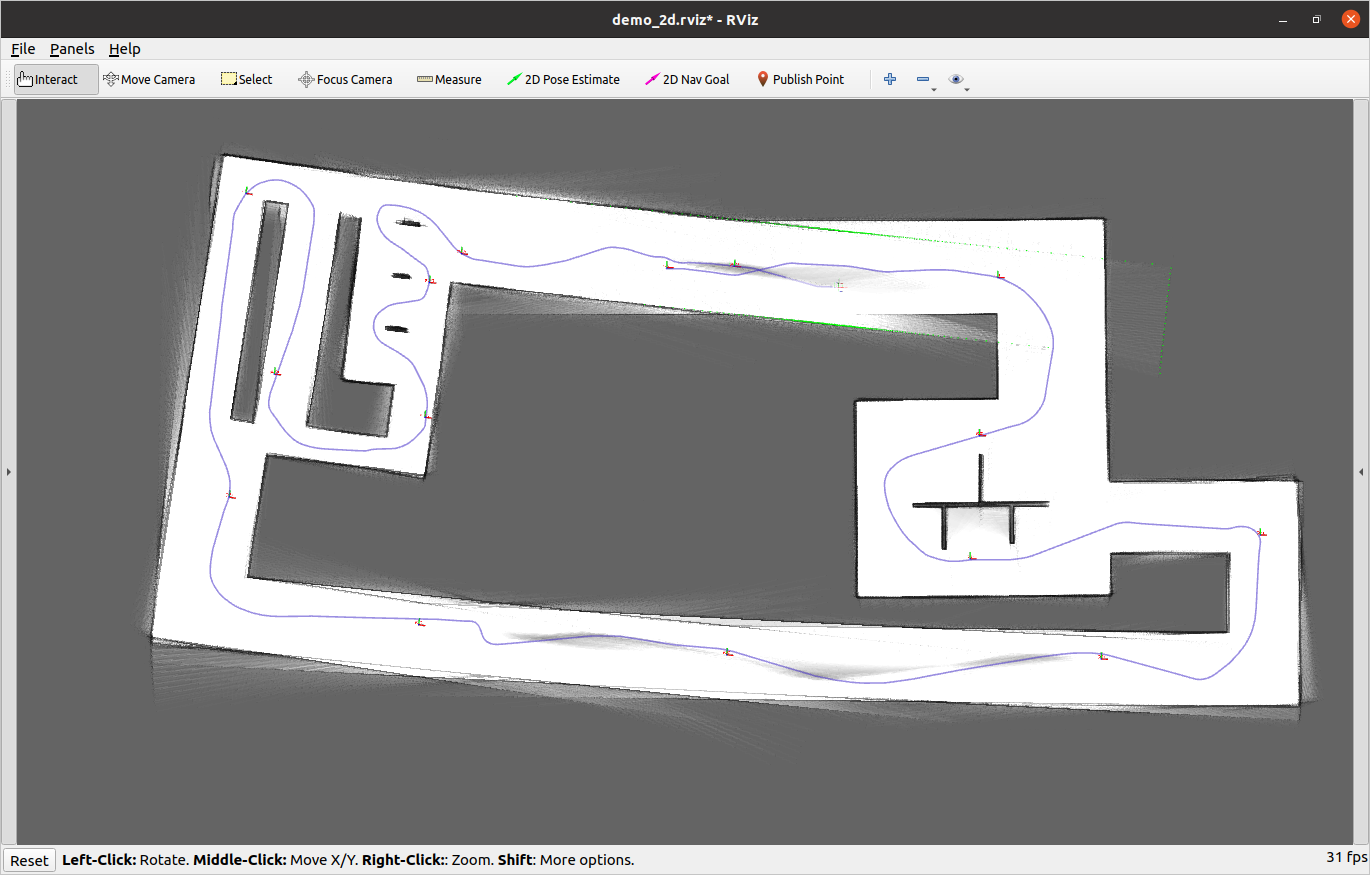
\includegraphics[width=5cm]{task3a_result2.png}
		\subcaption{After reaching the start point}
		\label{fig5b}
	\end{minipage}
	\begin{minipage}[t]{0.32\textwidth}
		\centering
		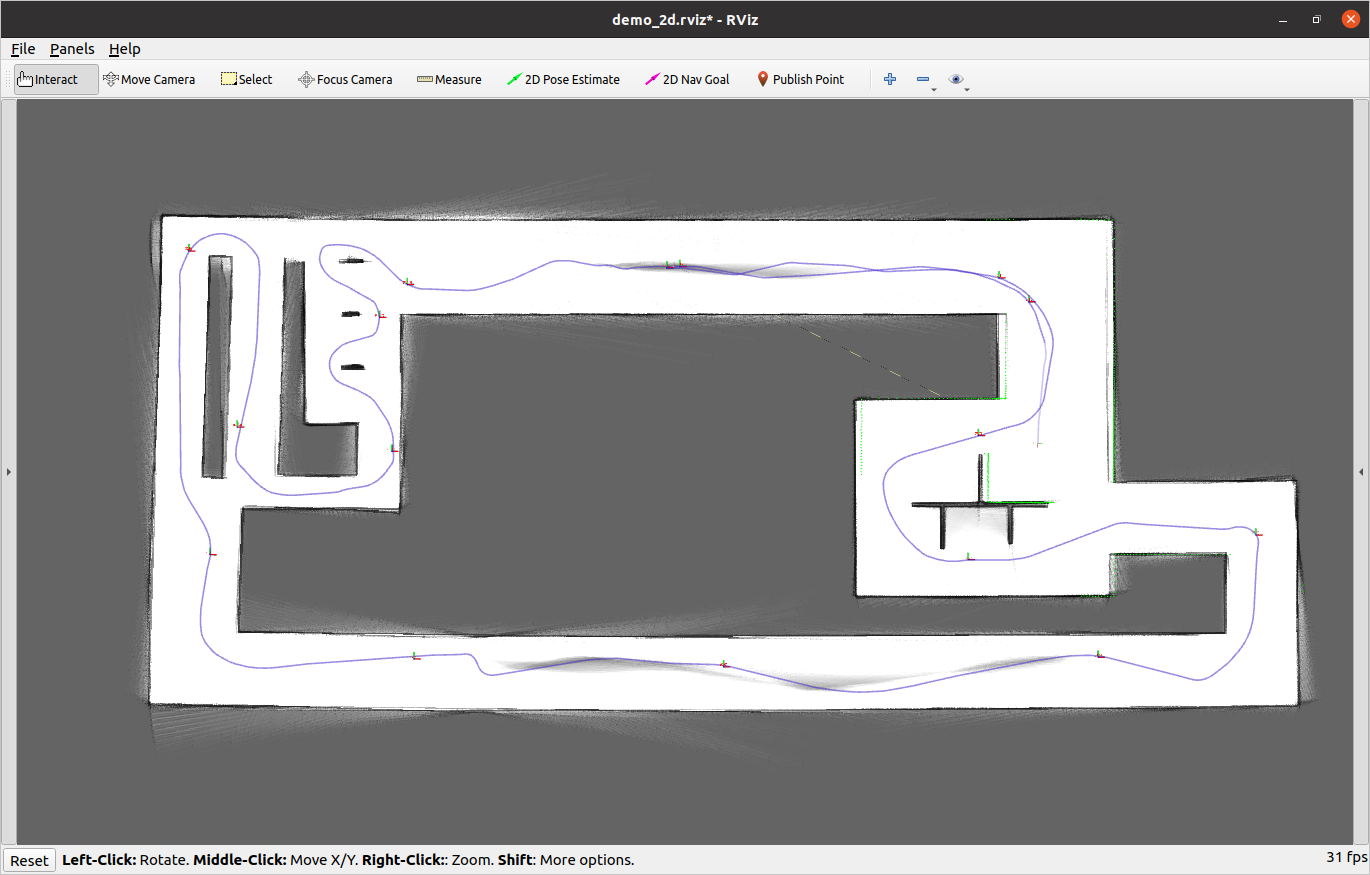
\includegraphics[width=5cm]{task3a_result3.png}
		\subcaption{Final mapping result}
		\label{fig5c}
	\end{minipage}
	\caption{2D LiDAR SLAM by Cartographer algorithm}
	\label{fig5}
\end{figure} 

We can see the map rotation is obvious since we have no IMU, we should give a lower rotation weight for ceres\_scan\_matcher. We also set minimum and maximum lidar range to be 0.3 and 100 respectively, and voxel filter size is set to be 0.02. Moreover, we find the loop closure is not stable, so we increase the min\_score of constraint\_builder to 0.7. The mapping results after tuning is shown in Fig.~\ref{fig6a}, where the performance looks slightly better than the former case. By the EVO tool, we plot the evaluation results in Fig.~\ref{fig6b}. We can see the maximum drift (2.737) appears after the robot reaches the start point, and the Absolute RMSE is 0.864 (Fig.~\ref{fig6c}), which is relatively good. 


\begin{figure}[H]
	\centering
	\begin{minipage}[t]{0.32\textwidth}
		\centering
		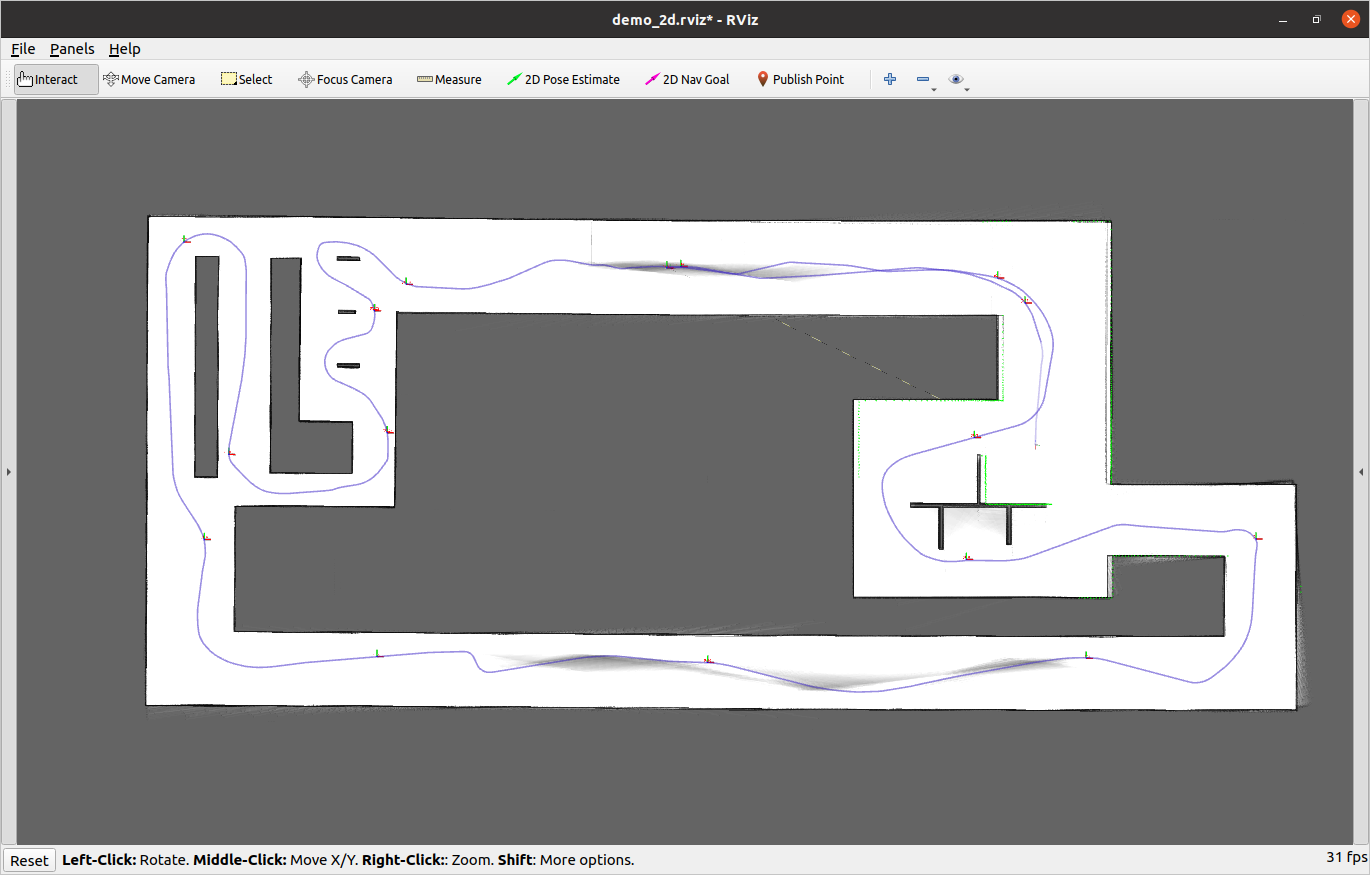
\includegraphics[width=5cm]{task3a_result4.png}
		\subcaption{Mapping results after tuning}
		\label{fig6a}
	\end{minipage}
	\begin{minipage}[t]{0.32\textwidth}
		\centering
		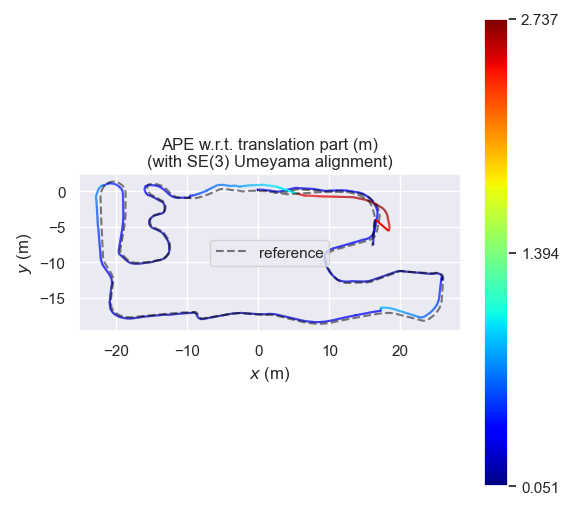
\includegraphics[width=5cm]{3a_evo2.png}
		\subcaption{Performance evaluation by EVO}
		\label{fig6b}
	\end{minipage}
	\begin{minipage}[t]{0.32\textwidth}
		\centering
		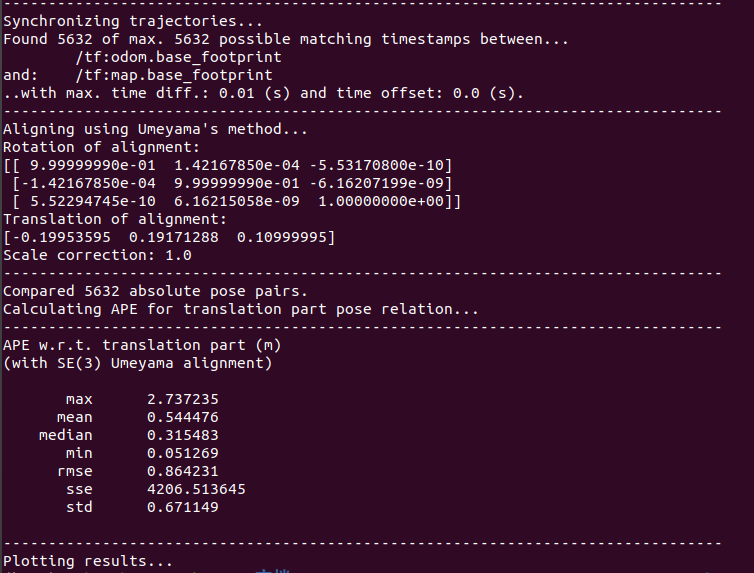
\includegraphics[width=5cm]{3a_evo3.png}
		\subcaption{Different metrics for evaluation}
		\label{fig6c}
	\end{minipage}
	\caption{Performance evaluation by EVO}
	\label{fig6}
\end{figure} 

One of the main disadvantages of Cartographer algorithm is that it requires a lot of computational resources, which can limit its use on low-power devices. Therefore, we may modify more parameters to achieve a lower latency. In addition, it can be challenging to configure and fine-tune so many hyper-parameters in Cartographer, and the "best" combination should be selected according to specific applications.

\subsection{A-LOAM for 3D LiDAR SLAM}

\hspace{1.0em}
In this task, we use the A-LOAM (3D LiDAR) algorithm to complete a 3D SLAM task on the given rosbag "3dlidar.bag". Here we refer this repo[1] to help do the task and directly generate odometry file for EVO evaluation.

The process of algorithm implementation can be concluded as:

\begin{itemize}[itemsep=3pt,topsep=0pt,parsep=0pt]
	\item[1.] Confirm system requirements: Ubuntu 20.04, ROS Noetic, C++14, CMake: 3.0.2 and above. 
	\item[2.] Install libraries required: Eigen3, PCL1.10, Ceres, evo.
	\item[3.] Develop the Aloam from repo into catkin\_ws (some modifications are needed which can be found in the ‘README.md’).
	\item[4.] Create a folder named ‘txt’, then copy the ground truth file ‘00.txt’ into folder and create a empty txt file ‘aloam.txt’ in folder.
	\item[5.] Launch the Aloam and then play the rosbag "3dlidar.bag" at the same time. The ‘aloam.txt’ in the txt file will store the Aloam lidar odometry result after finishing the Aloam algorithm.
	\item[6.] In ‘txt’ folder, evaluate the performance of the algorithm using EVO command "evo\_ape kitti 00.txt aloam.txt -r full -va --plot --plot\_mode xz".
\end{itemize}

Then, the result of the EVO evaluation of this 3D SLAM task is shown in Fig.~\ref{fig7}. 

\begin{figure}[H]
	\centering
	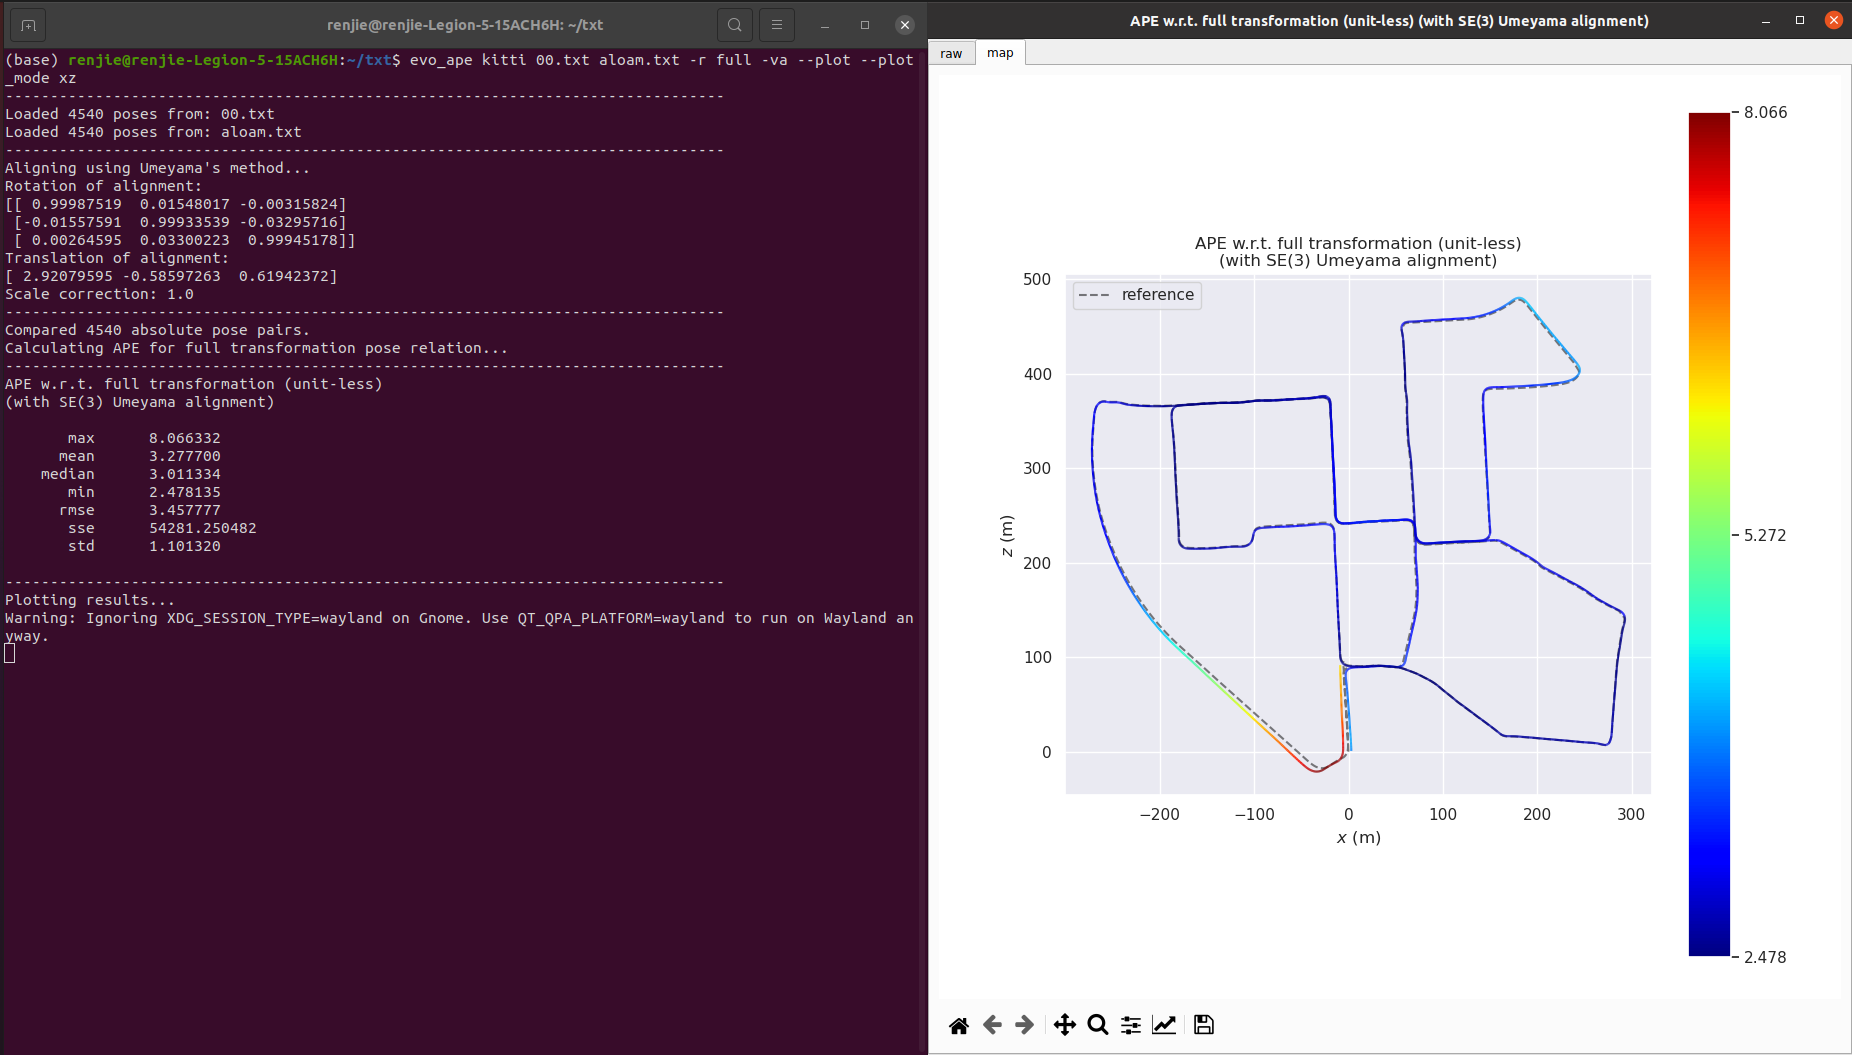
\includegraphics[width=8cm]{task3.1.b_result.png}
	\caption{3D SLAM task result}
	\label{fig7}
\end{figure}

Notice that in step 3, there are some modifications we did which the README.md do not mention. 

\begin{itemize}[itemsep=3pt,topsep=0pt,parsep=0pt]
	\item Firstly, it is needed to uncomment the “//generate the KITTI format trajectory result” part in the laserMapping.cpp, so that the Aloam lidar odometry result will be stored in ‘aloam.txt’. 
	\item Secondly, the ‘ceres::LocalParameterization’ and ‘ceres::EigenQuaternionParameterization’ are deprecated in the latest release of Ceres Solver (v 2.1.0) and need to be replaced to ‘ceres::Manifold’ and ‘ceres::QuaternionManifold()‘.
\end{itemize}

From the result, it can be seen that the max error value is 8.066, the mean error value is 3.278 and the min error value is 2.478. Thus, the performance of this algorithm is not bad.





\newpage

\bibliographystyle{IEEEtran}
%	
\bibliography{ref}{}

\citetext{1}{nuslde (2023) aloam\_lidar\_odom\_result\_generate}  \href{https://github.com/nuslde/aloam\_lidar\_odom\_result\_generate}{[Source Code]}

\begin{appendices}
	
	\section{Appendix}
	
	\textbf{\textcolor[rgb]{0.98,0.00,0.00}{my\_robot.lua}}
	\begin{figure}[H]
		\centering
		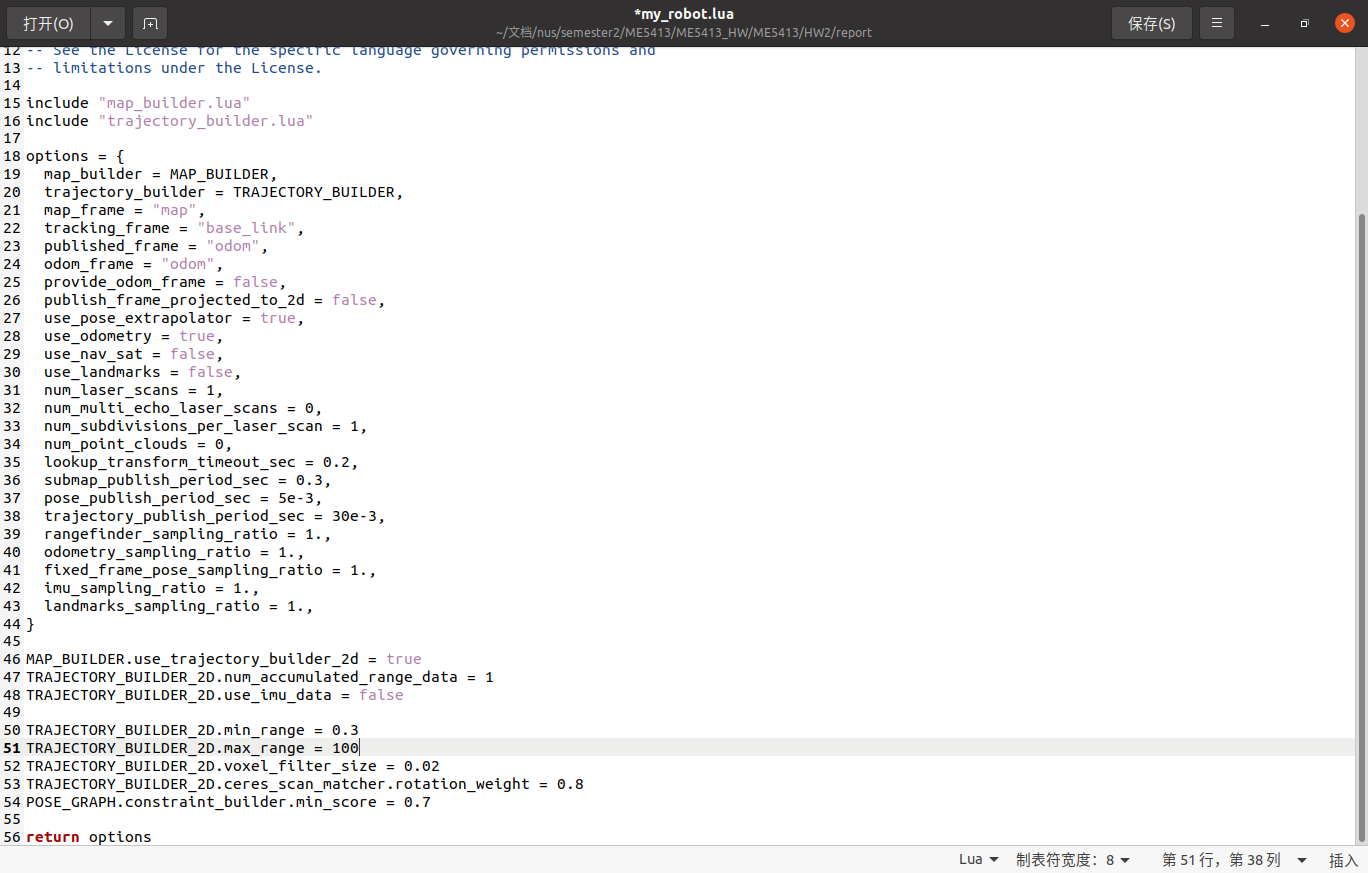
\includegraphics[width=18cm]{appendix2.png}
		\caption{my\_robot.lua}
	\end{figure} 

	
	\textbf{\textcolor[rgb]{0.98,0.00,0.00}{demo\_my\_robot.launch}}
	
	\begin{figure}[H]
		\centering
			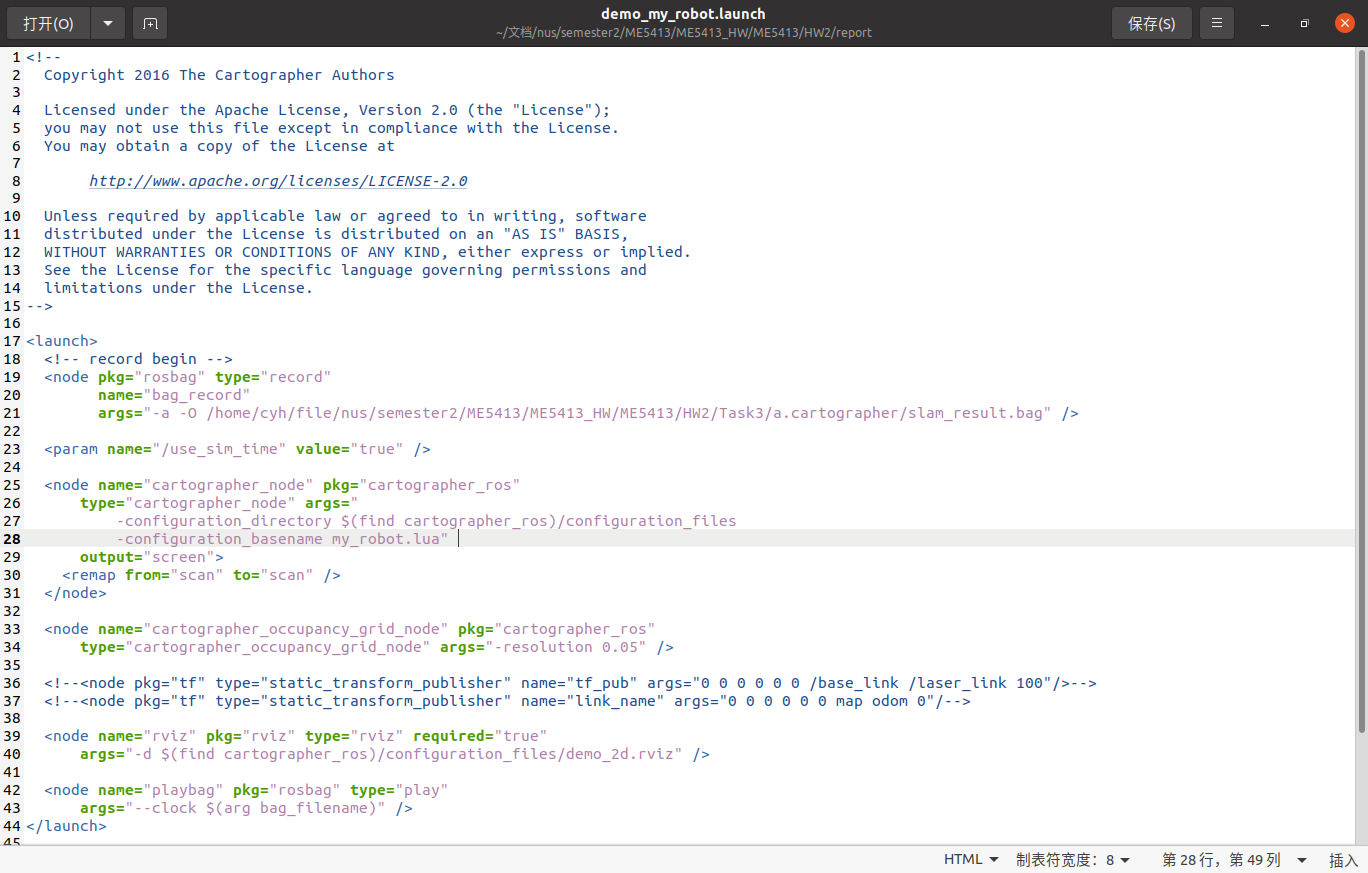
\includegraphics[width=18cm]{appendix1.png}
		\caption{demo\_my\_robot.launch}
	\end{figure} 
	

	
\end{appendices}



%\begin{appendices}
%	\section{xxx}
%	
%	\section{xxx}
%	
%\end{appendices}





	
\end{document}








